% !TEX root = CartaPerali_Report.tex
\section{Processing Pipeline}
\label{sec:processing_pipeine}

\noindent The code necessary to replicate this work is available in the GitHub repository \footnote{https://github.com/Fisher4537/HumanDataAnalitycs}.\\
The workflow used to implement the whole KWS system is depicted in Fig. \ref{fig:pipeline} \\
\begin{figure}[h]
			\centering
	    	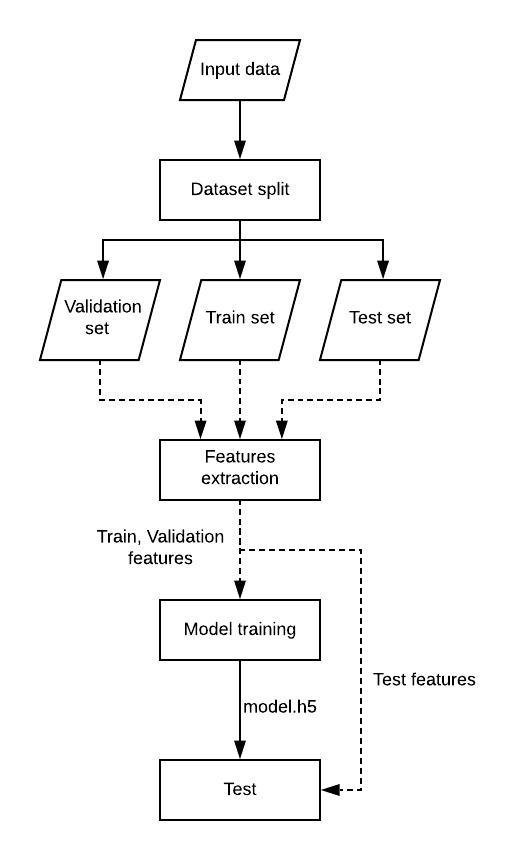
\includegraphics[width=6cm, height=8cm ,width=0.25\textwidth]{pipeline}
	    	\caption{System workflow}
	    	\label{fig:pipeline}
\end{figure} \\
\noindent As mentioned in the intro, the KWS system is trained on the '{\it{speech\_commands}}' dataset. The input dataset is split into {\it{train, test}} and {\it{validation}} and each one of them is then preprocessed and prepared for the features extraction task as described next.



\section{Data preprocessing and Features extraction}
\label{sec:model}

\noindent Data are preprocessed by mean of so called \mbox{{\it{"generators"}}} that are responsible for preparing batches of data containing the desired percentage of predefined wanted words, organized in a list, and the percentage of words that the model should classify as {\it {unknown}}. \\The following step is the extraction of relevant features from the audio signals. For this task, the MFCC coefficients are used. Mel-Frequency Cepstrum Coefficients (MFCC) frames are built using parameters depicted in Table \ref{table:mfcc_parameters}.
\begin{table}[h!]
\centering
\begin{tabular}{ p{3cm}|p{3cm}|}
\hline
Window length & 25ms \\
Frame shift  & 10ms  \\
N. Filterbanks & 26\\
N. FFT points & 512\\
\hline
\end{tabular}
\caption{MFCC parameters}
\label{table:mfcc_parameters}
\end{table}
\noindent In the end, one set of 13 MFCC coefficients is extracted from each frame.  Eventually the model will receive an input vector of the form (99, 13, 1).



\section{Learning Framework}
\label{sec:learning_framework}

\subsection*{\textbf {CNN architectures and training}}Processed input data contain at this point the feature vectors ready to fed as input to the model. \\ \\
%\begin{figure}[h]
%			\centering
%	    	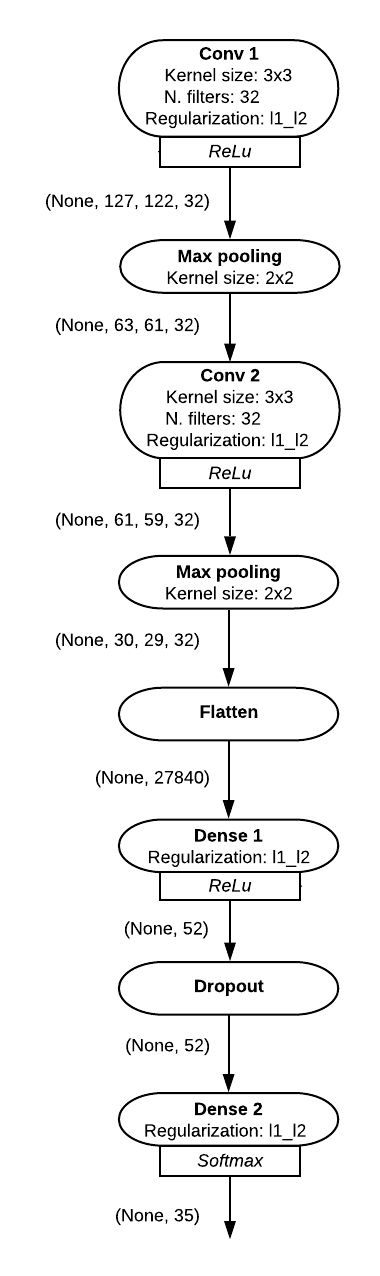
\includegraphics[width=5, height=8cm, width=0.25\textwidth]{CNN_schema}
%	    	\caption{CNN schema}
%	    	\label{fig:CNN_schema}
%\end{figure} 
\noindent 
\textbf{Model id: }mp.\\The first layer is a convolutional with a 3x3 kernel, 64x64 dimensional and ReLu activation function. The second layer is again a convolutional one with a 3x3 kernel, 32x32 dimensional and ReLu activation function. A flatten and a dense layer follow until a softmax function outputs a prediction. \\ \\ 
\textbf{Model id: }dd\_relu.\\ In this model ... \\ \\ 
\textbf{Model id: }dd\_drop.\\ In this model ... \\ \\ 
\textbf{Model id: }light\_cnn.\\ In this model ... \\ \\ 
\textbf{Model id: }light\_cnn\_reg\_2.\\ In this model ... \\ \\
\textbf{Model id: }light\_cnn\_reg\_drop.\\ In this model ... \\ 

The models are trained and optimized with two different built-in optimization algorithms in order to susequently compare the obtained results. The deployed optimizers are the classic Stochastic Gradient Descent (SGD) and the Adam algorithm. During the training of the model, several callbacks are passed as input to improve the performances in a computationally smart way. The {\it{ReduceOnPlateau}} callback takes care of setting the learning rate according to the behavior of the accuracy's curve; the {\it{EarlyStopping}} callback has the purpose to stop the training process, if no significant improvement is observed for a defined number of epochs. The {\it{TensorBoard}} callback function provides an interface to show the behavior of the metrics of interest during the training. In Fig. \ref{fig:CNN_loss} the behavior of the loss during the training phase is shown and in Fig.  \ref{fig:CNN_accuracy} accuracy's one is depicted.

\begin{figure}[h]
			\centering
	    	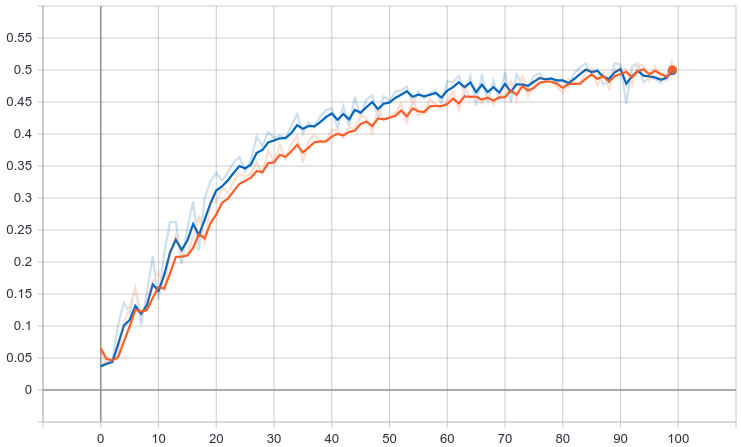
\includegraphics[width=8cm, height=6cm]{debug_tuy_acc}
	    	\caption{CNN training accuracy}
	    	\label{fig:CNN_accuracy}
\end{figure} 

\begin{figure}[h]
			\centering
	    	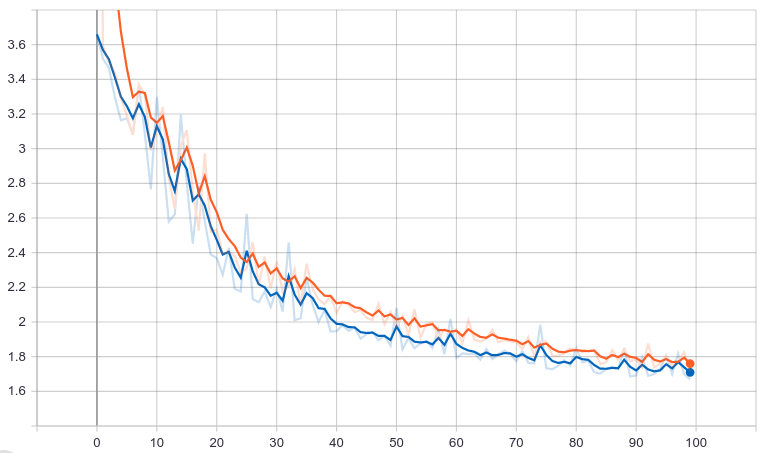
\includegraphics[width=8cm, height=6cm]{debug_tuy_loss}
	    	\caption{CNN training loss}
	    	\label{fig:CNN_loss}
\end{figure} 



